% !TeX root = ./Lecture2.tex
% created by Uwe Schadewald
% modified by Mathias Kuntze and Ahmet Uysal
% Add, handout to documentclass arguments for condensed pdf
\documentclass[presentation, 8pt, mathserif, t]{beamer} % , aspectratio=169
\usepackage[english]{babel}
\usepackage{pgf,graphicx}
\usepackage{amsmath, amssymb}
\usepackage[utf8]{inputenc}
\usepackage{lmodern}
\usepackage{palatino}
\usepackage{multimedia}
\usepackage{pgfpages} 
\usepackage{tikz}
\usepackage{datetime}
\pdfoptionpdfminorversion=5

\usepackage{caption}
\usepackage{subcaption}
% if else
\usepackage{ifthen}
% extend table options
\usepackage{tabularx} 
\usepackage{booktabs}
\usepackage{multicol}
\usepackage{multirow}
\usepackage{eso-pic}  % package to set background image
\usepackage[calc]{picture}

% Packages and stuff for ToDo list like itempoints
\usepackage{pifont}
\newcommand{\cmark}{\ding{51}}%
\newcommand{\xmark}{\ding{55}}%
\newcommand{\open}{$\square$}
\newcommand{\done}{\rlap{$\square$}{\raisebox{1pt}{\large\hspace{1.5pt}\cmark}}\hspace{-2.5pt}}
\newcommand{\wontfix}{\rlap{$\square$}{\raisebox{1pt}{\large\hspace{1.5pt}\xmark}}}
\newcommand{\notsure}{\rlap{$\square$}{\raisebox{0.8pt}{\large\hspace{1.5pt}\textbf{?}}}}



% side bar and footer
\setbeamertemplate{headline}{	
	\leavevmode
	\vspace{-4em}	
	\hbox{		
		\begin{beamercolorbox}[wd=0.85\paperwidth,ht=10ex,dp=8ex,center]{}%			
			% navigation with subsections as dots
			\hspace{3.5em}\insertnavigation{0.7\paperwidth}{\hskip0pt plus1fill} % add navigation in footer						
			% navigation with sections, no subsections
			% \insertsectionnavigationhorizontal{0.6\paperwidth}{\hskip0pt plus1fill}{} \\ % add navigation in footer}
			
		\end{beamercolorbox} 				
	}
	\vskip0pt
}


\setbeamertemplate{footline}{	
	\leavevmode
	\vspace{-3em}
	\hbox{
		\begin{beamercolorbox}[wd=.33\paperwidth,ht=2.25ex,dp=1ex,left]{author in head/foot}%
			\hspace{5em}
			\insertshortauthor
		\end{beamercolorbox}
		\begin{beamercolorbox}[wd=.33\paperwidth,ht=2.25ex,dp=1ex,center]{title in head/foot}%
			\insertshorttitle \ - \insertshortsubtitle
		\end{beamercolorbox}	
		\begin{beamercolorbox}[wd=0.30\paperwidth,ht=10ex,dp=8ex,right]{pagenumber in head/foot}			 	
			\insertframenumber % add page numbers
		\end{beamercolorbox}
	}			
	\vskip0pt
}



\setbeamertemplate{frametitle}{
	\ifthenelse{\equal{\insertframesubtitle}{}}{
		\vspace{0.6cm}
		\huge{\insertframetitle}
	}{
		\vspace{0.6cm}
		\small{\insertframetitle}\\
		\vspace{0.3cm}
		\huge{\insertframesubtitle}
    }		
}

	
% enumerate sections
\setbeamertemplate{section in head/foot}{\hfill\insertsectionheadnumber.~\insertsectionhead}
%\setbeamertemplate{section in head/foot shaded}{\color{structure!50}\hfill\insertsectionheadnumber.~\insertsectionhead}
\setbeamertemplate{section in toc}{\inserttocsectionnumber.~\inserttocsection}

%enumerate subsections
\setbeamertemplate{subsection in head/foot}{\hfill\insertsubsectionheadnumber.~\insertsubsectionhead}
\setbeamertemplate{subsection in head/foot shaded}{\color{structure!50}\hfill\insertsubsectionheadnumber.~\insertsubsectionhead}
%\setbeamertemplate{subsection in toc}[subsections numbered]
\setbeamertemplate{subsection in toc}{\vskip0.5em\leftskip=2em\inserttocsubsection\par}

%--------------------------Common------------------------------------------------------
\setbeamercovered{transparent} % make the beamer theme invisible
\usefonttheme{structurebold}
\beamertemplatenavigationsymbolsempty % set navigations helper function to off
\setbeamertemplate{bibliography item}[text]
\setbeamertemplate{note page}[plain]

%\setlist[itemize,1]{label={$\bullet$}} % \item are using bullets
\setbeamertemplate{itemize items}[circle]
	
	

	
% create a new command to show it on two screens
% I'm using dspdfviewer.
\newcommand{\setDualView} {
	\setbeameroption{show notes on second screen=right}
}

%\AtBeginSection[]{\subsection{}}
\newcommand{\addcite}[1]{%
	\AddToShipoutPictureFG*{%
		\AtPageLowerLeft{%
			\put(0.90\paperwidth,5em){											
				\tiny{
					\cite{#1} 
				}			
			}
		}
	}	
}

% insert a frame with references -> use bibtex
\newcommand{\insertReferenceFrame}[3]{%
	\section{#1}
	\begin{frame}[allowframebreaks]
		\frametitle{#1}
		\bibliographystyle{#2}
		\bibliography{#3}
	\end{frame}	
}

\AtBeginSection[]{\subsection{}}
	





\usepackage{../KU-Beamer-Template/style/koc}
\usepackage{minted}
\usepackage{upquote}
\usepackage{graphicx}
\usepackage{tikz}
\usetikzlibrary{shapes.symbols,positioning, chains}

% pdflatex --shell-escape Lecture2.tex & pdflatex --shell-escape Lecture2.tex

\title{KOLT Python}
\subtitle{Basic Operators, Intro to Branching \& Simple Functions}
\newdate{date}{04}{02}{2020}
\date{\displaydate{date}}
\author{Ceren Kocaoğullar}

\titlegraphic{
\includegraphics[scale=0.18]{../KU-Beamer-Template/style/images/kolt_logo.png}}

\setbeamercovered{invisible} % transparent
\makeatletter
\let\@@magyar@captionfix\relax
\makeatother
\begin{document}
    \maketitle

    \frame{\frametitle{Agenda}\tableofcontents}
    \section{Recap}
        \begin{frame}{Comments}
            \LARGE
            \inputminted[frame=single,framesep=2pt]{python3}{code-examples/comments.py}
            Python will basically ignore comments, they are purely written \textbf{for humans}!
        \end{frame}

        \begin{frame}{Variables}
            \LARGE
            \begin{table}[]
                \resizebox{0.8\textwidth}{!}{
                \begin{tabular}{|l|l|l|}
                \hline
                \textcolor{koc}{\textbf{Type}} &\textcolor{koc}{\textbf{Explanation}} & \textcolor{koc}{\textbf{Examples}} \\ \hline
                \textbf{\texttt{int}}  & represent \textbf{integers} & 3, 4, 17, -10 \\ \hline
                \textbf{\texttt{float}} & represent \textbf{real numbers} & 3.0, 1.11, -109.123123 \\ \hline
                \textbf{\texttt{bool}} & represent \textbf{boolean} truth values & \texttt{True}, \texttt{False} \\ \hline
                \textbf{\texttt{str}} & A sequence of characters. & \textquotesingle Hello\textquotesingle, \textquotesingle \textquotesingle, \textquotesingle 3\textquotesingle \\ \hline
                \textbf{\texttt{NoneType}}& special and has one value, None & \texttt{None} \\ \hline
                \end{tabular}}
            \end{table}

            \begin{itemize}
                \item How to create a variable?
                \texttt{variable\_name = value}
                \item How about types?
                use \texttt{type()}
                \item Can a variable change type?
                \textbf{Yes!} Just assing a new value with any type.
                \item What if we if want to convert a value between types, i.e, \textquotesingle 2\textquotesingle $\to$ 2?
            \end{itemize}
        \end{frame}

        \begin{frame}{Casting}
            \LARGE
            \begin{itemize}
                \item \texttt{int(\textquotesingle 2\textquotesingle)} $\to$ 2
                \pause
                \item Any possible reasons for casting?
                \pause
                \begin{itemize}
                    \LARGE
                    \item Taking user input\\
                    \item Reading numbers from a file\\
                \end{itemize}
                \pause
                \item Can we cast every value to every type?
                \\
                \pause
                \textbf{NO!}
                \\try \texttt{int(\textquotesingle hello\textquotesingle)}
            \end{itemize}
        \end{frame}

        \begin{frame}{Console I/O(Input/Output)}
            \huge
            \textbf{\texttt{print(*args, sep=\textquotesingle \ \textquotesingle, end=\textquotesingle \textbackslash n\textquotesingle )}}
            \begin{itemize}
                \LARGE
                \item Can take arbitrary number of arguments
                \item Separates elements with space by default
                \item Adds newline character \texttt{\textquotesingle \textbackslash n\textquotesingle} to end by default
            \end{itemize}

            \textbf{\texttt{input([prompt])}}
            \begin{itemize}
                \LARGE
                \item Prints the prompt to Console
                \item Program is paused until user enters something
                \item \textbf{returns an \texttt{str} object!}
            \end{itemize}
        \end{frame}


     \section{Basic Operators}
        \begin{frame}{Arithmetic Operators}
            \LARGE
            These operations are applicable on Numeric types: \texttt{int} and \texttt{float}
            \pause
            \begin{columns}
               \begin{column}{0.40\textwidth}
                \vspace{-5mm}
                \begin{itemize}
                    \item \texttt{+}: Addition
                    \pause
                    \item \texttt{-}: Subtraction
                    \pause
                    \item \texttt{*}: Multiplication
                    \pause
                    \item \texttt{/}: Division
                    \pause
                    \item \texttt{//}: Floor (integer) Division
                    \pause
                    \item \texttt{\%}: Modulo
                    \pause
                    \item \texttt{**}: Power
                \end{itemize}
               \end{column}
               \pause
               \begin{column}{0.65\textwidth}
                \inputminted[frame=single,framesep=2pt]{python3}{code-examples/numeric_operators.py}
               \end{column}
            \end{columns}
        \end{frame}

        \begin{frame}{Assignment Operators}
            \LARGE
            We have already seen \texttt{\textquotesingle=\textquotesingle}:
            \texttt{variable\_name = value}\\
            \pause
            \\
            Frequently we will update variables' values based on their \textbf{old value}.\\
            \textbf{Ex:} Increment a number: \texttt{num = num + 1}\\
            \pause
            \\
            Python has shorter representations for these updates with arithmetic operators.\\
            \pause
            \texttt{num += 1} is equivalent to \texttt{num = num + 1}\\
            \pause
            \texttt{result *= 2} is equivalent to \texttt{result = result * 2}\\
        \end{frame}

        \begin{frame}[c]{Assignment Operators}
            \LARGE
			\begin{table}[]
				\resizebox{0.7\textwidth}{!}{
				\begin{tabular}{|l|l|l|}
				\hline
				\textcolor{koc}{\textbf{Operator}} &\textcolor{koc}{\textbf{Usage}} & \textcolor{koc}{\textbf{Equivalent}} \\ \hline
				\textbf{\texttt{+=}} & \texttt{val += 3} & \texttt{val = val + 3} \\ \hline
				\textbf{\texttt{-=}} & \texttt{val -= 3} & \texttt{val = val - 3} \\ \hline
				\textbf{\texttt{*=}} & \texttt{val *= 3} & \texttt{val = val * 3} \\ \hline
				\textbf{\texttt{/=}} & \texttt{val /= 3} & \texttt{val = val / 3} \\ \hline
                \textbf{\texttt{\%=}}& \texttt{val \%= 3} & \texttt{val = val \% 3} \\ \hline
                \textbf{\texttt{**=}} & \texttt{val **= 3} & \texttt{val = val ** 3} \\ \hline
				\textbf{\texttt{//=}} & \texttt{val //= 3} & \texttt{val = val // 3} \\ \hline
				\end{tabular}}
			\end{table}
        \end{frame}

        \begin{frame}{\texttt{bool} Operators}
            \LARGE
            How to represent logical operations in Python?
            \begin{table}[]
                \resizebox{0.45\textwidth}{!}{
                \begin{tabular}{|c|c|c|c|c|}
                \hline
                \textcolor{koc}{\textbf{A}} &\textcolor{koc}{\textbf{B}} & \textcolor{koc}{\textbf{A or B}} & \textcolor{koc}{\textbf{A and B}} & \textcolor{koc}{\textbf{not A}}\\ \hline
                \textbf{\texttt{True}}  & \textbf{\texttt{True}}  & \textbf{\texttt{True}}  & \textbf{\texttt{True}} & \textbf{\texttt{False}} \\ \hline
                \textbf{\texttt{True}} & \textbf{\texttt{False}}  & \textbf{\texttt{True}} & \textbf{\texttt{False}} & \textbf{\texttt{False}} \\ \hline
                \textbf{\texttt{False}} & \textbf{\texttt{True}}  & \textbf{\texttt{True}} & \textbf{\texttt{False}} & \textbf{\texttt{True}} \\ \hline
                \textbf{\texttt{False}} & \textbf{\texttt{False}} & \textbf{\texttt{False}} & \textbf{\texttt{False}} & \textbf{\texttt{True}} \\ \hline
                \end{tabular}}
            \end{table}
            \pause
            \begin{columns}[c]
                \column{0.25\textwidth}
                    \begin{itemize}
                        \item \textbf{\texttt{and}}
                        \pause
                        \item \textbf{\texttt{or}}
                        \pause
                        \item \textbf{\texttt{not}}
                    \end{itemize}
                \pause
                \column{0.75\textwidth}
                    \texttt{True or False and False} $\Rightarrow$
                    \pause
                    \textbf{\texttt{True}} \\
                    \pause
                    \medskip
                    \Huge
                    \textbf{WHY?}
            \end{columns}

        \end{frame}

        \begin{frame}{Operator Precedence}
            \LARGE
            Logical operators are evaluated in this order:
            \begin{enumerate}
                \item \texttt{not}
                \item \texttt{and}
                \item \texttt{or}
            \end{enumerate}
            \pause
            \medskip
            You can override this order with parentheses\\
            \pause
            \smallskip
            \texttt{(True or False) and False} $\Rightarrow$
            \pause
            \textbf{\texttt{False}} \\
        \end{frame}

        \begin{frame}{Short-Circuit Evaluation}
            \LARGE
            \texttt{X}: Any boolean value\\
            \texttt{True or X} $\Rightarrow$
            \pause
            \textbf{\texttt{True}}\\
            \pause
            \texttt{False and X} $\Rightarrow$
            \pause
            \textbf{\texttt{False}}\\
            \pause
            Python is smart enough to take advantage of this!
            \pause
            \medskip
            \inputminted[frame=single,framesep=2pt]{python3}{code-examples/short_circuit.py}
        \end{frame}

        \begin{frame}[c]{Truthy \& Falsy Values}
            \begin{columns}
                \column{0.45\textwidth}
                    \inputminted[firstline=1, lastline=8, frame=single,framesep=2pt]{python3}{code-examples/truthy-falsy.py}
                \pause
                \column{0.54\textwidth}
                    \inputminted[firstline=9, lastline=16, frame=single,framesep=2pt]{python3}{code-examples/truthy-falsy.py}
            \end{columns}
        \end{frame}

        \begin{frame}{Comparison Operators}
            \LARGE
            \begin{columns}[c]
                \begin{column}{0.4\textwidth}
                    \begin{itemize}
                        \item \texttt{<}: Strictly less than
                        \pause
                        \item \texttt{<=}: Less than or equal
                        \pause
                        \item \texttt{>}: Strictly greater than
                        \pause
                        \item \texttt{>=}: Greater than or equal
                        \pause
                        \item \texttt{==}: Equal
                        \pause
                        \item \texttt{!=}: Not equal
                    \end{itemize}
                \end{column}
                \pause
                \begin{column}{0.6\textwidth}
                    \inputminted[frame=single,framesep=2pt]{python3}{code-examples/comparison.py}
                \end{column}
            \end{columns}
        \end{frame}

        \begin{frame}{Chained Comparisons}
            \LARGE
            \texttt{1 < 2 < 3} $\Rightarrow$
            \pause
            \textbf{\texttt{True}}\\
            \pause
            You can chain arbitrarily many comparison operations together.\\
            \pause
            $v_{i}$: variables/values, $op_{i}$: comparison operators\\
            \pause
            \texttt{$v_{1}\ op_{1}\ v_{2}\ op_{2}\ v_{3}\ ...\ op_{n-1}\ v_{n}$} is equivalent to:\\
            \texttt{$v_{1}\ op_{1}\ v_{2}$ \textbf{and} $v_{2}\ op_{2}\ v_{3}$ \textbf{and} ...$v_{n-1}\ op_{n-1}\ v_{n}$}\\
            \pause
            \vspace{-4mm}
            \inputminted[frame=single,framesep=2pt]{python3}{code-examples/chained.py}
        \end{frame}

    \section{Branching}
        \begin{frame}{Branching}
            \pause
            \begin{center}
                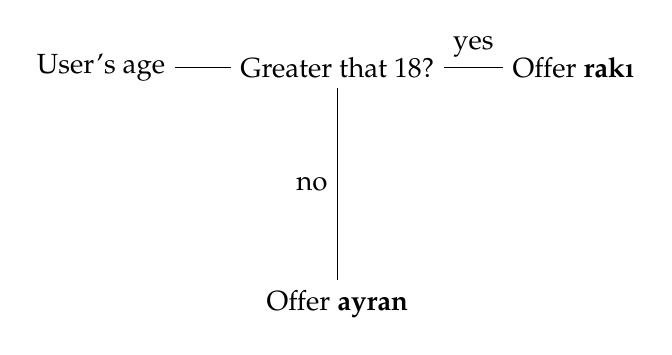
\begin{tikzpicture}[node distance=2cm]
                    \node (in1) {User's age};
                    \node (dec1) [right of=in1, xshift=1cm] {Greater that 18?};
                    \node (proc1) [right of=dec1, xshift=1cm] {Offer \textbf{rakı}};
                    \node (proc2) [below of=dec1, yshift=-1cm] {Offer \textbf{ayran}};
                    \draw (in1) -- (dec1);
                    \draw (dec1) -- node[anchor=south] {yes} (proc1);
                    \draw (dec1) -- node[anchor=east] {no} (proc2);
                \end{tikzpicture}
                \\
                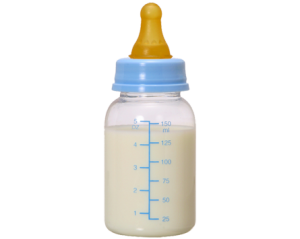
\includegraphics[width=0.25\textwidth]{Lecture2/images/milk_bottle.png}
                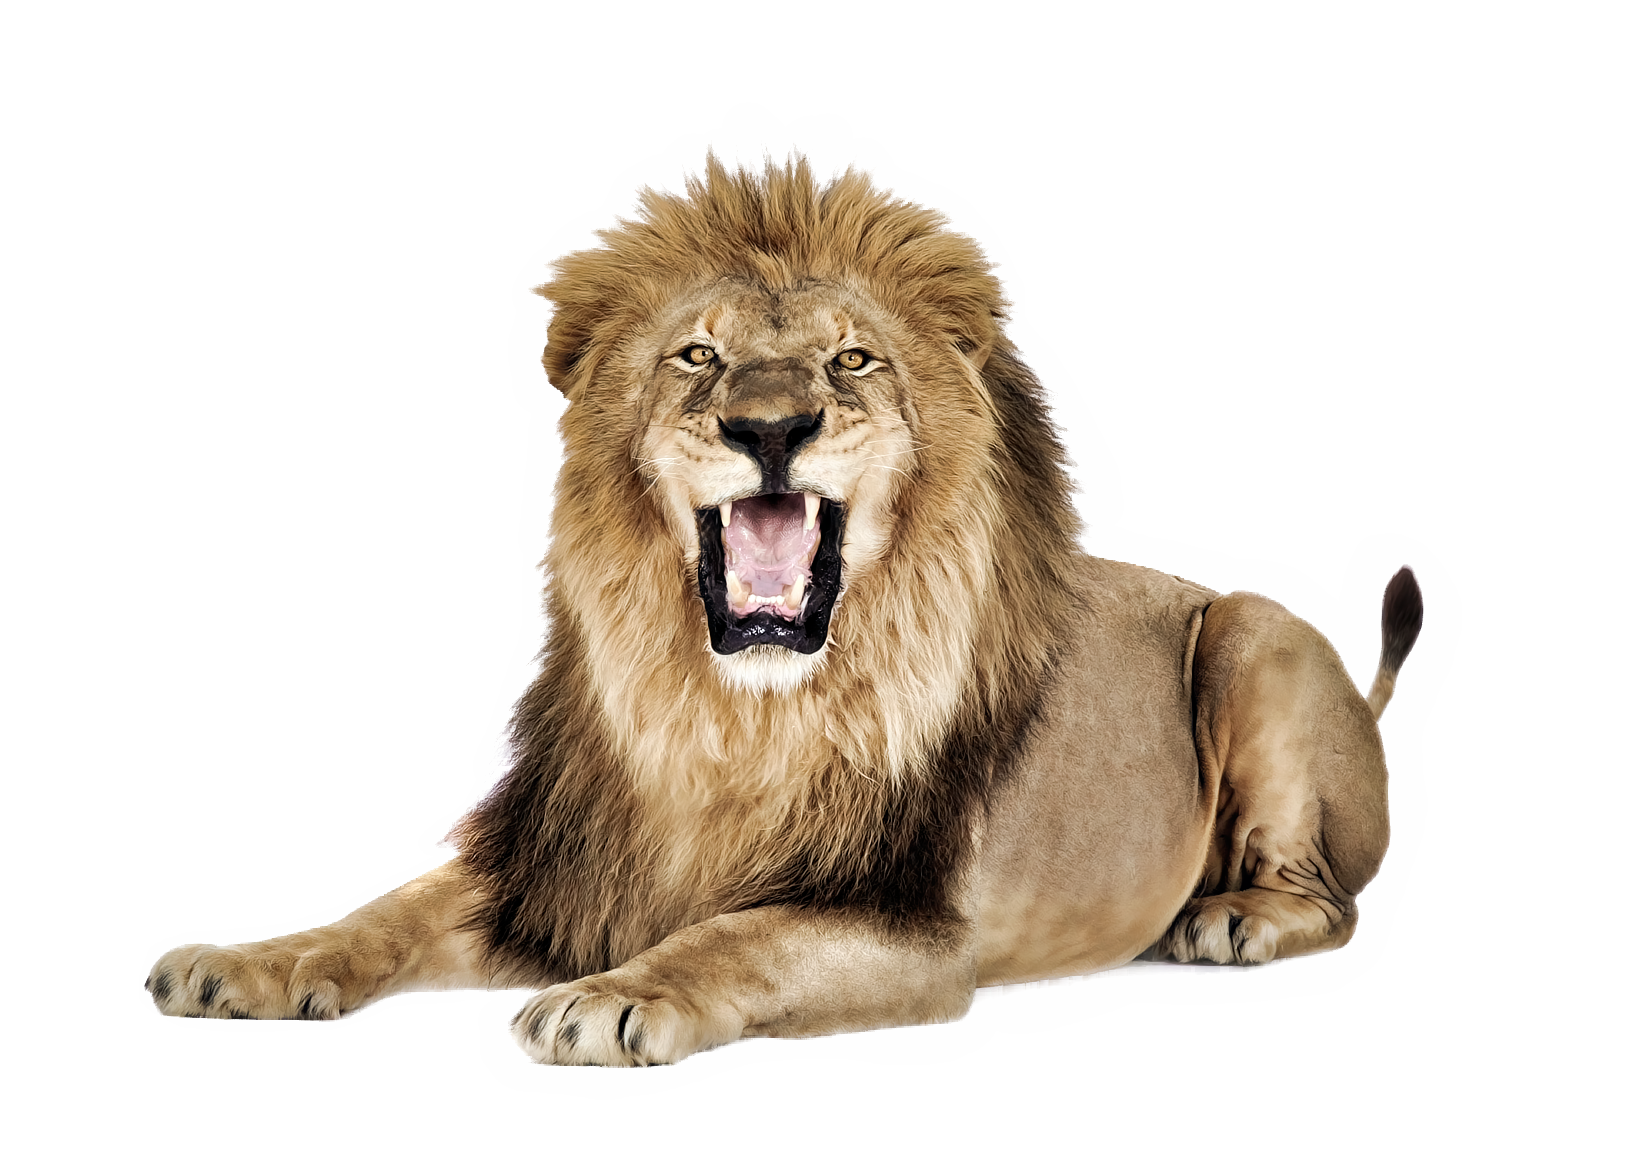
\includegraphics[width=0.25\textwidth]{Lecture2/images/lion.png}
                
\includegraphics[width=0.15\textwidth]{Lecture2/images/ayran.png}
            \end{center}
        \end{frame}

        \begin{frame}{Branching}
            \vspace{-3mm}
            \begin{columns}
                \column{0.5\textwidth}
                \inputminted[firstline=1, lastline=4, frame=single,framesep=2pt]{python3}{code-examples/branching.py}
                \inputminted[firstline=6, lastline=13, frame=single,framesep=2pt]{python3}{code-examples/branching.py}
                \column{0.5\textwidth}
                \inputminted[firstline=15, lastline=27, frame=single,framesep=2pt]{python3}{code-examples/branching.py}
            \end{columns}
            \begin{itemize}
                \item \texttt{<condition>} has a \textbf{\texttt{bool}} value (\texttt{True} or \texttt{False})
                \item Which expressions will be evaluated in which conditions?
            \end{itemize}
        \end{frame}

    \section{Objects}
        \begin{frame}[c]{Python Data Model}
            \pause
            \LARGE
            How did we represent data in Python?\\
            \\
            \pause
            \textbf{Variables!}\\
            \pause
            \\
            How do they work?\\
            \pause
             Do they store the data themselves?
            \pause
        \end{frame}

    \begin{frame}{Objects}
        \LARGE
        \textbf{Everything} is an object in Python.
        \\
        \begin{columns}
            \begin{column}[c]{0.5\textwidth}
                \LARGE
                \visible<4->{\texttt{a = 5}\\}
                \visible<8->{\texttt{a = 10}\\}
                \visible<12->{\texttt{a += 3}\\}
                \visible<16->{\texttt{print(a)}}
            \end{column}
            \begin{column}[c]{0.5\textwidth}
                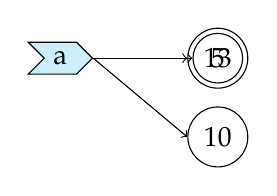
\begin{tikzpicture}%[node distance=-0.15mm]
                    \visible<6->{\node[signal, draw, signal from=west, fill=cyan!20] (var1) {a};}
                    \visible<5-10>{\node[circle, draw, right of=var1, shift={(1,0)}] (val1) {5};}
                    \visible<7-9>{\draw[->] (var1.east) -- (val1.west);}
                    \visible<9-14>{\node[circle, draw, below of=val1] (val2) {10};}
                    \visible<10-13>{\draw[->] (var1.east) -- (val2.west);}
                    \visible<13->{\node[circle, draw, right of=var1, shift={(1,0)}] (val3) {13};}
                    \visible<14->{\draw[->] (var1.east) -- (val3.west);}
                \end{tikzpicture}
           \end{column}
       \end{columns}
       \medskip
        $\hookrightarrow$ Values at the right side of our label analogy are
        objects!\\
        \pause
         Even though variables \textbf{do not} have \texttt{types}, each object has a \textbf{fixed} \texttt{type}.
    \end{frame}

    \begin{frame}[c]{Objects - Identity}
        \Large
        Each object has an \texttt{identity},
        \pause
         this value can be obtained by using \texttt{\textbf{id()}} function.\\
        \pause
        \\
        \textbf{==} operator compares values \\\textbf{\texttt{is}} operator compares identities
        \pause
    \end{frame}

    \begin{frame}{Objects - Identity}
        \begin{center}
            \Large
            Is this glass half full or half empty?
            \\
            
\includegraphics[width=0.30\textwidth]{Lecture2/images/glass.png}
            \pause
            \inputminted[frame=single,framesep=2pt, firstline=6]{python3}{code-examples/identity.py}
            \pause
        \end{center}
    \end{frame}

    \section{Basic Functions}
        \subsection{Defining Functions}
        \begin{frame}[c]{Functions}
            \LARGE
            Functions are blocks of
            \pause
            \textbf{organized},
            \pause
            \textbf{reusable} code
            \pause that carry some \textbf{specific} tasks.\\
            \pause
            \begin{center}
                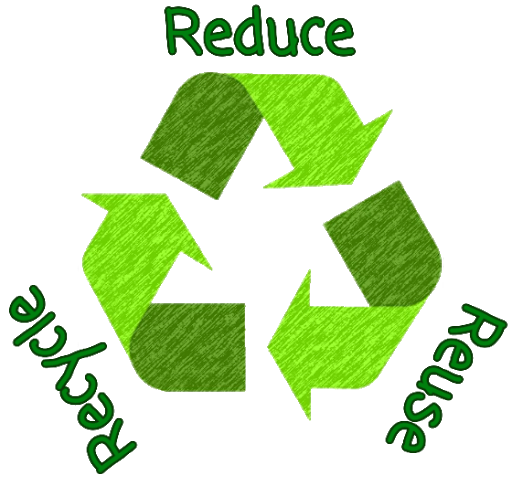
\includegraphics[width=0.3\textwidth]{Lecture2/images/reduce_reuse_recycle.png}
            \end{center}
        \end{frame}

        \begin{frame}[c]{Functions}
            \large
            \textbf{Menemen \textit{without} Onions}
            \normalsize
            \inputminted[firstline=1, lastline=4, frame=single,framesep=2pt]{python3}{code-examples/menemen.py}
            \pause
            \large
            \textbf{Menemen \textit{with} Onions}
            \normalsize
            \inputminted[firstline=6, lastline=11, frame=single,framesep=2pt]{python3}{code-examples/menemen.py}
            \pause
            \begin{center}
            \begin{tikzpicture}[remember picture,overlay]
                \node[xshift=65mm,yshift=-48mm] at (current page.north west){%
                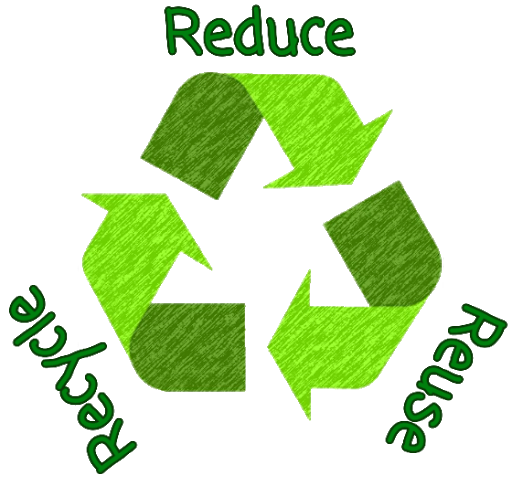
\includegraphics[width=0.5\textwidth]{Lecture2/images/reduce_reuse_recycle.png}};
            \end{tikzpicture}
            \end{center}
        \end{frame}

        \begin{frame}{Defining Functions}
            \LARGE
            \textbf{\texttt{def}} keyword introduces a function \textbf{\textit{definition}}.
            \\
            \large
            \inputminted[firstline=14, lastline=16, frame=single,framesep=2pt]{python3}{code-examples/menemen.py}
            \inputminted[firstline=18, lastline=20, frame=single,framesep=2pt]{python3}{code-examples/menemen.py}
        \end{frame}

        \begin{frame}{Functions}
            \LARGE
            \textit{Defining} a \texttt{function} only makes it available.\\
            \pause
            You should \textit{call} the \texttt{function} to execute it.\\
            \pause
            \\
            \large
            \textbf{Menemen \textit{without} Onions}
            \inputminted[firstline=32, lastline=33, frame=single,framesep=2pt]{python3}{code-examples/menemen.py}
            \pause
            \textbf{Menemen \textit{with} Onions}
            \inputminted[firstline=35, lastline=38, frame=single,framesep=2pt]{python3}{code-examples/menemen.py}
            \begin{center}
            Defining a function = \textbf{writing down the recipe}\\
            Calling a function = \textbf{executing the recipe}
            \end{center}
        \end{frame}

        \begin{frame}{Functions}
            \LARGE
            You \textbf{can} call a function inside another function.\\
            \pause
            \large
            \inputminted[firstline=22, lastline=24, frame=single,framesep=2pt]{python3}{code-examples/menemen.py}
            \pause
            \inputminted[firstline=26, lastline=30, frame=single,framesep=2pt]{python3}{code-examples/menemen.py}
        \end{frame}
\end{document}
